\section{The Riemann Problem}
\label{sec:riemann-problem}

Sections~\ref{sec:nonuniqueness}--\ref{sec:entropy-condition} treated the
specific data $u_\ell=0<u_r=1$. This section gives the complete entropy
solution for arbitrary constant states $u_\ell, u_r \in \mathbb{R}$, i.e.
the general \emph{Riemann problem}
\begin{equation}
  \label{eq:general-riemann-data}
  u_0(x) = \begin{cases} u_\ell, & x<0, \\ u_r, & x>0. \end{cases}
\end{equation}

\subsection{The rarefaction fan}
\label{subsec:rarefaction-general}

The solution $u_B(x,t)=x/t$ constructed in
Section~\ref{subsec:nonuniq-rarefaction} is a special case of a
\emph{self-similar} solution, i.e. one of the form $u(x,t)=g(x/t)$.
Writing $\xi = x/t$ and substituting into the PDE gives
\begin{equation}
  u_t + u\,u_x = -\frac{\xi}{t}g'(\xi) + \frac{g(\xi)}{t}g'(\xi)
  = \frac{g'(\xi)}{t}\big(g(\xi)-\xi\big) = 0,
\end{equation}
so any self-similar solution satisfies either $g'(\xi)=0$ (a constant
state) or $g(\xi)=\xi$ (the fan $u=x/t$) on each interval of $\xi$. This
is exactly the structure needed to connect two constant states, provided
$u_\ell < u_r$: since characteristic speed equals $u$, the states
$u_\ell$ and $u_r$ correspond to characteristics of speed $u_\ell$ and
$u_r$, and the fan $u=x/t$ smoothly interpolates the speeds in between
whenever $u_\ell<u_r$.

\subsection{The complete solution}
\label{subsec:riemann-complete}

\begin{theorem}[Entropy solution of the Riemann problem]
\label{thm:riemann-solution}
The unique entropy solution of \eqref{eq:ivp} with data
\eqref{eq:general-riemann-data} is:
\begin{enumerate}
  \item[\textup{(a)}] If $u_\ell > u_r$ (shock case),
  \begin{equation}
    \label{eq:riemann-shock}
    u(x,t) = \begin{cases} u_\ell, & x < st, \\ u_r, & x > st, \end{cases}
    \qquad s = \frac{u_\ell+u_r}{2}.
  \end{equation}
  \item[\textup{(b)}] If $u_\ell \leq u_r$ (rarefaction case),
  \begin{equation}
    \label{eq:riemann-rarefaction}
    u(x,t) = \begin{cases}
      u_\ell, & x \le u_\ell t, \\
      x/t, & u_\ell t < x < u_r t, \\
      u_r, & x \ge u_r t.
    \end{cases}
  \end{equation}
\end{enumerate}
\end{theorem}

\begin{proof}
\emph{(a)} As in Proposition~\ref{prop:shock-is-weak-solution}, $u$ is
locally constant away from $x=st$ and jumps at the Rankine--Hugoniot
speed $s=(u_\ell+u_r)/2$ across it, so $u$ is a weak solution by
Theorem~\ref{thm:rankine-hugoniot}. Since $u_\ell>u_r$, the Lax condition
\eqref{eq:lax-burgers} holds, so $u$ is an entropy solution; uniqueness is
Theorem~\ref{thm:oleinik-uniqueness}.

\emph{(b)} The case $u_\ell=u_r$ is the trivial constant solution, so
suppose $u_\ell<u_r$. On each of the three regions in
\eqref{eq:riemann-rarefaction}, $u$ is $C^1$ and solves the PDE
classically: on the outer two by inspection, and on the fan
$u_\ell t<x<u_r t$ by Section~\ref{subsec:rarefaction-general}. At the two
interior boundaries $x=u_\ell t$ and $x=u_r t$, $u$ is continuous (both
one-sided limits agree, equalling $u_\ell$ and $u_r$ respectively), so
exactly as in Proposition~\ref{prop:rarefaction-is-weak-solution} the
boundary terms in the weak formulation vanish and $u$ is a weak solution.
It contains no jump discontinuity, so it is vacuously an entropy
solution, and uniqueness is again Theorem~\ref{thm:oleinik-uniqueness}.
\end{proof}

Taking $(u_\ell,u_r)=(0,1)$ in case (b) recovers exactly $u_B$ from
Section~\ref{subsec:nonuniq-rarefaction}, and taking $(u_\ell,u_r)=(1,0)$
in case (a) gives the shock $s=1/2$ analogous to $u_A$ --- now correctly
identified as the entropy solution, since the roles of $u_\ell$ and $u_r$
are reversed from Section~\ref{sec:nonuniqueness} and the Lax condition
\eqref{eq:lax-burgers} now holds.

\begin{figure}[h]
\centering
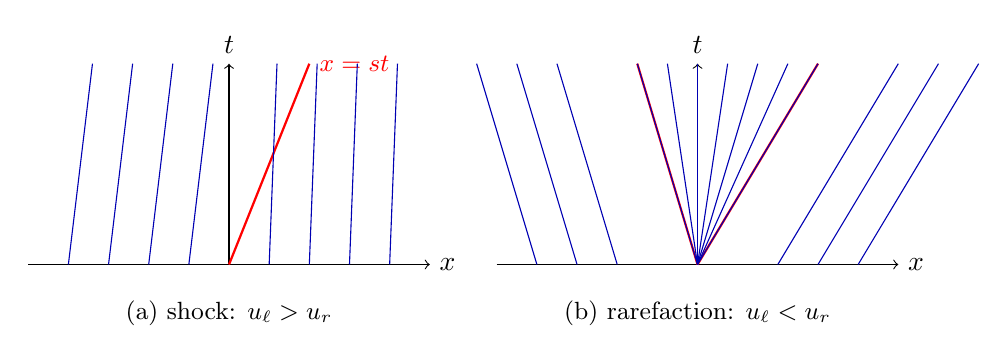
\begin{tikzpicture}[scale=0.85]
  % --- Shock case (left) ---
  \begin{scope}
    \draw[->] (-3,0) -- (3,0) node[right] {$x$};
    \draw[->] (0,0) -- (0,3) node[above] {$t$};
    \draw[thick, red] (0,0) -- (1.2,3) node[right] {\small $x=st$};
    \foreach \xz in {-2.4,-1.8,-1.2,-0.6}{
      \draw[blue!70!black] (\xz,0) -- ({\xz+0.4*3*0.3},3);
    }
    \foreach \xz in {0.6,1.2,1.8,2.4}{
      \draw[blue!70!black] (\xz,0) -- ({\xz+0.13*3*0.3},3);
    }
    \node[below] at (0,-0.4) {\small (a) shock: $u_\ell>u_r$};
  \end{scope}
  % --- Rarefaction case (right) ---
  \begin{scope}[xshift=7cm]
    \draw[->] (-3,0) -- (3,0) node[right] {$x$};
    \draw[->] (0,0) -- (0,3) node[above] {$t$};
    \draw[thick, red] (0,0) -- (-0.9,3);
    \draw[thick, red] (0,0) -- (1.8,3);
    \foreach \xz in {-2.4,-1.8,-1.2}{
      \draw[blue!70!black] (\xz,0) -- ({\xz-0.3*3},3);
    }
    \foreach \m in {0,1,...,6}{
      \draw[blue!70!black] (0,0) -- ({-0.9+\m*0.45},3);
    }
    \foreach \xz in {1.2,1.8,2.4}{
      \draw[blue!70!black] (\xz,0) -- ({\xz+0.6*3},3);
    }
    \node[below] at (0,-0.4) {\small (b) rarefaction: $u_\ell<u_r$};
  \end{scope}
\end{tikzpicture}
\caption{Characteristic pictures for the two cases of
Theorem~\ref{thm:riemann-solution}. (a) Characteristics from both sides
converge into the shock curve $x=st$. (b) Characteristics fan out from
the origin, filling the gap left by the diverging characteristics from
$u_\ell$ and $u_r$.}
\label{fig:riemann-characteristics}
\end{figure}